 \documentclass{article}
\usepackage{graphicx} % Required for inserting images
\usepackage{listings}
\usepackage{xcolor}
\usepackage{url}
\usepackage{hyperref}

\definecolor{codegreen}{rgb}{0,0.6,0}
\definecolor{codegray}{rgb}{0.5,0.5,0.5}
\definecolor{codepurple}{rgb}{0.58,0,0.82}
\definecolor{backcolour}{rgb}{0.95,0.95,0.92}

\lstdefinestyle{mystyle}{
    backgroundcolor=\color{backcolour},   
    commentstyle=\color{codegreen},
    keywordstyle=\color{magenta},
    numberstyle=\tiny\color{codegray},
    stringstyle=\color{codepurple},
    basicstyle=\ttfamily\footnotesize,
    breakatwhitespace=false,         
    breaklines=true,                 
    captionpos=b,                    
    keepspaces=true,                 
    numbers=left,                    
    numbersep=5pt,                  
    showspaces=false,                
    showstringspaces=false,
    showtabs=false,                  
    tabsize=2
}

\lstset{style=mystyle}

\title{Mandatory Assignment 1, INF226}
\author{Lars Haukland}
\date{September 2023}

\begin{document}

\maketitle

\section{Task 00}

For this task we are delivered the ELF file 00 and the source code for it.
Here is the source code for the ELF, this will be important for later:
\lstinputlisting[language=C]
{00.c}

\subsection{Vulnerability}
Well the vulnerability here, as in all of the tasks is that the program is vulnerable to a buffer overflow attack. Important to \textbf{NOTE} that the reason it is vulnerable to a buffer overflow is because the fgets takes in more bytes that the buffer is in size and assigns it to the buffer.\\
If we read the source code we can see that the program only outputs the flag if the check variable in the struct locals, line 8, is equal to "0x00c0ffee".
Since we are lucky that the developer put the buffer array together with the check variable in the same struct we know that these will be in the same order in the Stack frame. We can also double check this by using the provided tool on \url{inf226.puffling.no/frames}. If we type into the terminal \lstinline{frames 00} then we get the stack frame:\\
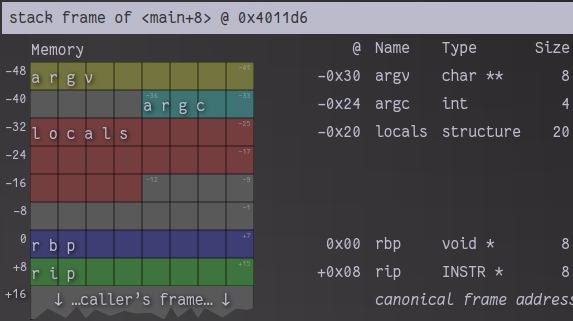
\includegraphics[scale=0.5]{stackframe-00.png} \\
From this we can see that the only thing we need to do is fill the buffer and input 0x00c0ffee.

It will also be useful to note the type of locals.check, it is a 32bit int.

\subsection{Code}

\lstinputlisting[language=Python]
{solve00.py}

\subsection{Explanation of code}

Here we do as describet in the Vulnerability section but here is a step by step:\\ \\
Import pwntools. Line 1\\ \\
open connection to the server on port 7000. Line 4 \\ \\
send 16 bytes plus the hex value "0x00c0ffee" as a 32 bit integer \\ \\
shutdown the output, this makes it so we can send data without the new line at the end (\textbackslash n). Line 10 \\ \\
print the output from the server (flag). Line 13


\subsection{Flag}
INF226\{s33kret c0de\}

\subsection{How could it be avoided?}
There are to areas of improvement I can see with the limited lectures we've had up to this point in INF226. That is to \begin{enumerate}
    \item Not have the buffer and check variable in the same struct. As this makes it so that they are guaranteed to be stored next to each other in the stack.
    \item Not allow fgets to read more bytes than the buffer is in size. In this case fgets reads up to 512 bytes and puts them in the buffer, but the buffer is only 16 bytes in size.
\end{enumerate}

\section{Task 01}
For this task we are delivered the ELF file 01 and the source code for it.
Here is the source code for the ELF, this will be important for later:
\lstinputlisting[language=C]
{01.c}
\subsection{Vulnerability}
In this task it is quite similar to 00 but different in that we now have a pointer instead of a 32 bit integer, vars.funPointer. The type of this pointer is volatile int which we can interpret as a 64 bit integer. Again the buffer, of size 16 this time, and funPointer are in a struct called vars. This guarantees they are placed by eachother in the stack. We can verify this by usig the same tool as in 00. \lstinline{frames 01} gives us: \\
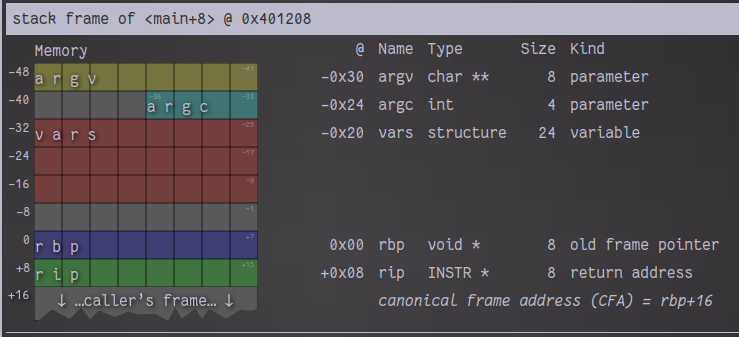
\includegraphics[scale=0.5]{stackframe-01.png} \\
From this we see that locals in total is 24 bytes. This confirmes our assumption because the buffer is 16 bytes and then the funPointer is $24 - 16 = 8$ bytes, or 64 bits.
Now from the source code we can see that once this vars.funPointer has been overwritten and is no longer NULL as assigned on line 18, the code calls vars.funPointer on line 28.
In the code we can also see that there is a function getFlag, and that this flag outputs the flag with a system call. It is a system call because the flag is stored on the server and not in the code. \\
With this information we know that we want to call getFlag to make the program output the flag. All we need to do then is to find the memory adress of that function so that we can override vars.funPointer to become that address.\\
To find the address we can use objdump, we write \lstinline{objdump -d 01} and get a lot of information but here is a screenshot of the memory address to getFlag:\\
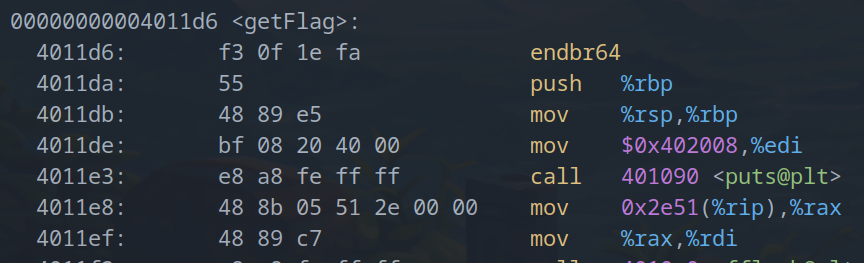
\includegraphics[scale=0.5]{objdump-01.png}\\
From this, we can see that the address starts with a bunch of 0s and then 4011d6. We can shorten the address to 0x4011d6 for hex. And now we have a plan: \\
Overflow 16-byte buffer and insert 0x4011d6 as a 64-bit integer so that it points to getFlag.\\
This will call getFlag and output the flag. \\ \\

\textbf{REMEMBER} The big reason we can do this buffer overflow attack is because the fgets takes in more bytes than the buffer is in size and then assigns it to the buffer. fgets takes in 512 bytes when the buffer is 16.

\subsection{Code}
\lstinputlisting[language=Python]
{solve01.py}
\subsection{Explanation of code}
The explanation from Vulnerability should be enough but here is a step-by-step: \\
Import pwntools. Line 1 \\
Open connection to the server on port 7001 \\ \\
Send 16 bytes and then the address to getFlag as a 64-bit integer \\ \\
Shutdown output so that we don't send a newline \\ \\
Read the flag. \\ \\
This overflows the buffer and makes vars.funPointer into the adress of getFlag so that the program then calls getFlag.

\subsection{Flag}
INF226\{d3 h0ly gra1l\}

\subsection{How could it be avoided?}
\subsection{How could it be avoided?}
There are to areas of improvement I can see with the limited lectures we've had up to this point in INF226. That is to \begin{enumerate}
    \item Not have the buffer and funPointer variable in the same struct. As this makes it so that they are guaranteed to be stored next to each other in the stack.
    \item Not allow fgets to read more bytes than the buffer is in size. In this case fgets reads up to 512 bytes and puts them in the buffer, but the buffer is only 16 bytes in size.
\end{enumerate}


\section{Task 02}
For this task, we are delivered the ELF file 02 and the source code for it.
Here is the source code for the ELF, this will be important for later:
\lstinputlisting[language=C]
{02.c}

\subsection{Vulnerability}
This program is also vulnerable to a bufferflow attack. For the same reason as the previous, fgets allocate more bytes to the buffer than the buffer is in size. This program is different from the previous, as it does not contain a variable that needs to be some certain value for the program to output the flag, and the buffer is not stored in a struct. This program also takes in two inputs, first one that is assigned to the buffer and then another one that is assigned to the buffer. The interesting part happens in between these inputs. There is some calculation and then the program outputs a pointer to the buffer plus some offset, the value of this offset is atoi (buffer). Atoi is a function in c that just converts a string to an integer. \\
In this task the hint together with the first string of the program "What is the carrying capacity of a domestic canary ? " are some pretty big hints.\\
The canary here in the first output refers to a stack canary. A stack canary is just an integer that is placed on the stack, just between the variables in the program and the return pointers, as a security measure against buffer overflow attacks. When running the program, if the stack canary value is changed the program knows that a buffer overflow attack is taking place and exits the program with the message **stack smashing detected**. \\
We can sort of see the stack canary in the stackframe but the previous tool for stackframes won't tell us it is the canary. Here is the stackframe after giving \lstinline{frames 02}: \\
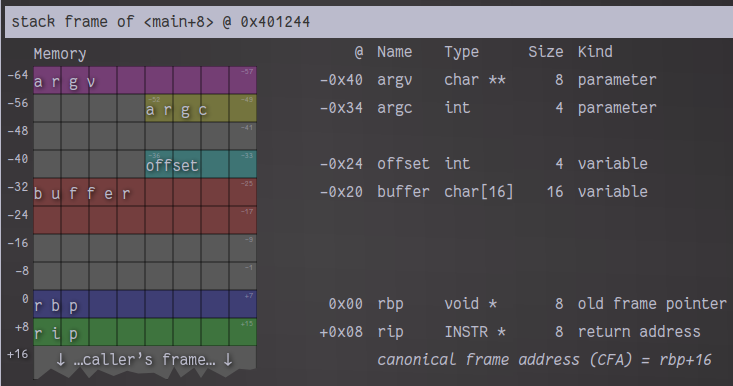
\includegraphics[scale=0.5]{stackframe-02.png} \\
We can see that after the buffer 16 bytes are unknown. Stack canaries are normally 64 bits on 64-bit architecture which I assume the server is running as there are few 32-bit computers left. \href{https://security.stackexchange.com/a/149136}{This answers confirm this.}\\ \\
So with this information, we know that 8 of these bytes have to be the canary. \\
We also know that we need to keep this canary value when overflowing. \\
Now I observed in all the other tasks that the canary always was on -8 in the stackframe and confirmed this with Anya over discord. Because of this, my first instinct is that the stack canary are the 8 bytes in -8. This padding of 8 bytes on -16 might indicate that the stack is aligned which we will solve later.
\\ \\
Now we know enough to crack this elf but how you may ask. Well we know that based on our input a value is then outputted based on a pointer to address, we do not need to understand this math to calculate the address. Now we want this pointer to point to the canary, this way the program will give us the canary value and we can overflow the buffer, then keeping the canary on the stack and then overflowing the return pointer so that it points to getFlag and the program runs the getFlag function. Here comes the code I used and then explanation of that code.
\\\\
Note that again this exlpoit is only possible because the fgets actually takes in more bytes than the buffer is in size and then assigns all the bytes to that buffer.
\subsection{Code}
\textbf{Program 1, finding the canary offset}
\lstinputlisting[language=Python]
{findOffset.py}
\textbf{Program 2, executing exploit}
\lstinputlisting[language=Python]
{solve02.py}
\subsection{Explanation of code}
\textbf{Program 1}\\
Here in program 1, I find the canary offset. We already know the offset from looking at the stack frame but it didn't hurt to check :D. I find out that the offset is 24 bytes. Hence if we give the 24 bytes as input we will hit the canary so anything above this will override the canary and crash the program.
\\ \\
\textbf{Program 2} \\
This program is the one to crack the elf.\\
From the hint text "What is the carrying capacity of a domestic canary?" my instinct was to input 24 after finding out that that was the offset. And let me just say that I was lucky, because after testing this it turns out the program ends up with the canary address after the calculation and it is outputted as the hint after 24 is given (as bytes of course). 
\\ \\
So as you probably can see the first part of the program just opens the connection, sends 24 as bytes and then retrieves the hint value from the program. And now comes the payload. The first parts are good, we fill the buffer and offset with 24 bytes and then give the canary value. The functions here first turns the hex value from the hint into an integer and then using p64 to format it as an 8 byte integer. We then give another 8 bytes, this is to skip the rbp cause we want to override the rip so that the program returns into the getFlag function.
\\ \\
Then now comes the part where we need to think about stack alignment... \\
Here is the objdump of 02, \lstinline{objdump -d 02}: \\
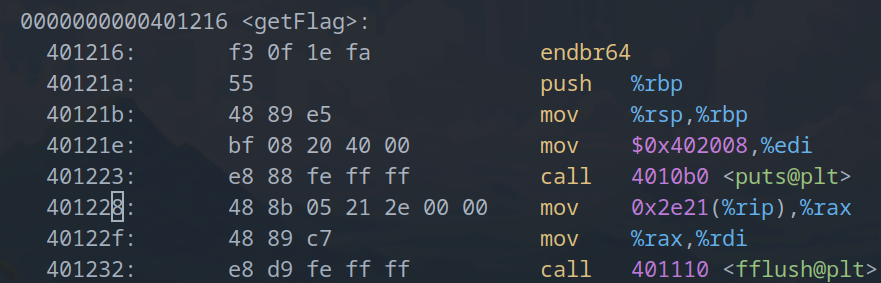
\includegraphics[scale=0.5]{objdump-02.png} \\
Now our instincts are to just point straight to the getFlag address \lstinline{0x401216} but this will make the program print out "Congrats! you can get the flag" and then stop. This is because the stack is aligned and a very detailed problem not covered. For more information I will refer to the course wiki that said "The precise reason for this is somewhat complicated (and you don't need to understand it); some instructions (in particular the SSE/AVX vector instructions that use the XMM registers) require addresses to be aligned on a 16-byte boundary (more details in the lecture or in this stack overflow answer)." You can find it \href{https://git.app.uib.no/inf226/23h/inf226-23h/-/wikis/lectures/ROP#solving-the-system-crash}{here}. That wiki explains that we need to point 5 bytes down, or just below the instruction push \%rbp. This is the adress \lstinline{0x40121b}.

With all this we make the return pointer point back to the getFlag function and the flag is printed out. We use \lstinline{io.shutdown('out)} just to avoid sending a new line character. And then read the flag with \lstinline{print(io.readall())}.

\subsection{Flag}
INF226\{s3r1nu5\_s3r1nu5\}

\subsection{How could it be avoided?}
Here there is only one point of improvement that I see to this program. And that is, like before, that fgets reads more bytes than the buffer is in size (512 vs 16). There is also this weird way of printing a hint, and of course if this hint wasn't being printed and leaking the canary value then it would be much harder to crack.

\section{Task 03}
For this task, we are delivered the ELF file 03 and the source code for it.
Here is the source code for the ELF, this will be important for later:
\lstinputlisting[language=C]
{03.c}
\subsection{Vulnerability}
The vulnerability is again that the program is vulnerable to a buffer overflow attack. Again this is by large because of fgets allocating more bytes to the buffer than the buffer is in size. The reason this task is harder than the previous ones are because this elf has PIE enabled. PIE stand for Position Independent Executable and means that the binary is position independent and can be put anywhere in the memory. Luckily for us the server opens it as a child process everytime we connect, this makes it so the position is independent and not the same as our pc but the same on the server everytime. Therefor all we need to do is bruteforce that address of the main stack.
\\ \\
Instead of trying to find the address of the stack I figured why not just try to find the address of the stack canary as this program also has a canary. But how would we know when we find the canary? Well we have this unsigned long* line\_pointer, and while yes it is set to point to the address of the variable line (line 17) we can still override it and make it point to the canary. Therefore, if we bruteforce the address of the canary and then overflow the buffer to make the line\_pointer variable point to the canary, the program will output the canary value (line 27). Then with this canary we overflow the buffer, include the canary and make the RIP point to, you guessed it, the getFlag function! Now again this stack frame is aligned somehow so we need to skip the push \%rbp instruction in getFlag, here is the objdump of getFlag: \lstinline{objdump -d 03} \\
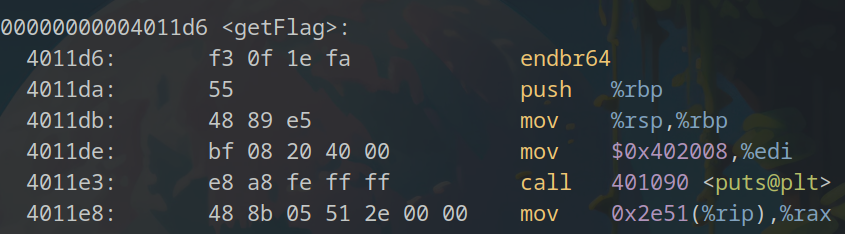
\includegraphics[scale=0.5]{objdump-03.png} \\
yes I changed my background while doing the assignment so this screenshot has that new background :)\\
\\
Now from the image we can see that instead of pointing to the address 0x4011d6 we need to point to the address 0x4011db so that we skip the push \%rbp instruction.
\\ \\
Now I have skipped alot of the introductional info as I wrote in the other tasks. But we can look at the stack frame here aswell if we want: \lstinline{frames 03} \\
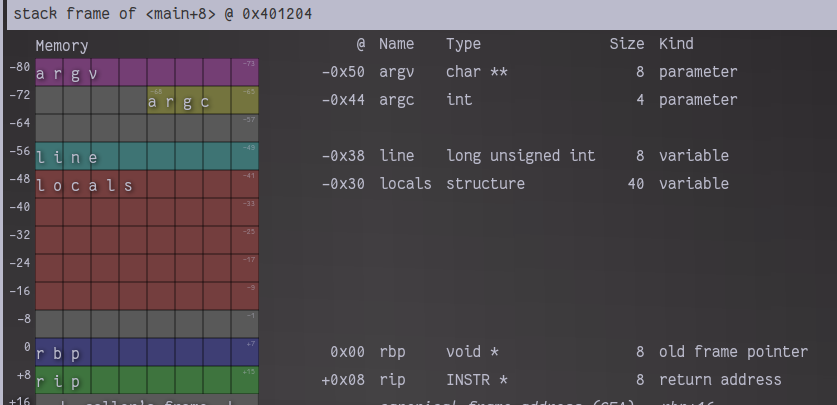
\includegraphics[scale=0.5]{stackframe-03.png} \\
This stackframe is not as interesting anymore as we are quite familiar with how this looks from the previous tasks. The buffer is 32 bytes and the line\_pointer is 8 bytes so this makes locals 40 bytes. And it is quite obvious that the uknown 8 bytes after locals is the canary.
\subsection{Code}
\lstinputlisting[language=Python]
{solve03.py}
\subsection{Explanation of code}
You may wonder how I just came up with the address range for the for loop but this was actually a tip in the task, and the step of the for loop could probably be 8 bytes but I chose to go for 4 just in case :). So the code pretty simply loops through all the addresses tries to overflow the buffer and point to the address. If the address is not the address of the canary then the program will close with stack smashing when we try to override the RIP and then an exception will occur, thats why we have a try and except.\\ \\
Its important to note the sendline after the payload is sent to override the RIP (line 25) because if we dont do this the while loop in the ELF will not stop. We will have succeeded with the attack but without this input of "\textbackslash n" it would not exit the while loop. \\
Then we check, if the program did not fail, is the flag in the output. If so then we know we hit the right canary and we can stop the program and the loop.
\subsection{Flag}
INF226\{cr3p3s r g00d\}

\subsection{How could it be avoided?}
There are to areas of improvement I can see with the limited lectures we've had up to this point in INF226. That is to \begin{enumerate}
    \item Not have the buffer and line\_pointer variable in the same struct. As this makes it so that they are guaranteed to be stored next to each other in the stack.
    \item Not allow fgets to read more bytes than the buffer is in size. In this case fgets reads up to 128 bytes and puts them in the buffer, but the buffer is only 32 bytes in size.
\end{enumerate}

There is also the fact that this hack would not work in a modern system as a modern system uses ASLR. This makes it so that the address of the canary would be different everytime and we could not bruteforce it, because if we tried event guessing the program would terminate right away.

\end{document}
